\chapter{Лабораторная работа}

\section*{Масштаб проекта}

Группа из 8 чел., длительность не более 4 мес., бюджет не более 620 тыс. руб.

\section*{Задание 1: Настройка рабочей среды проекта}

Установим дату начала проекта:

\begin{figure}[H]
	\begin{center}
		
\includegraphics[width=0.7\textwidth]{imgs/task_1_0.png}
	\end{center}
\end{figure}

Установим настройки расписания:

\begin{figure}[H]
	\begin{center}
		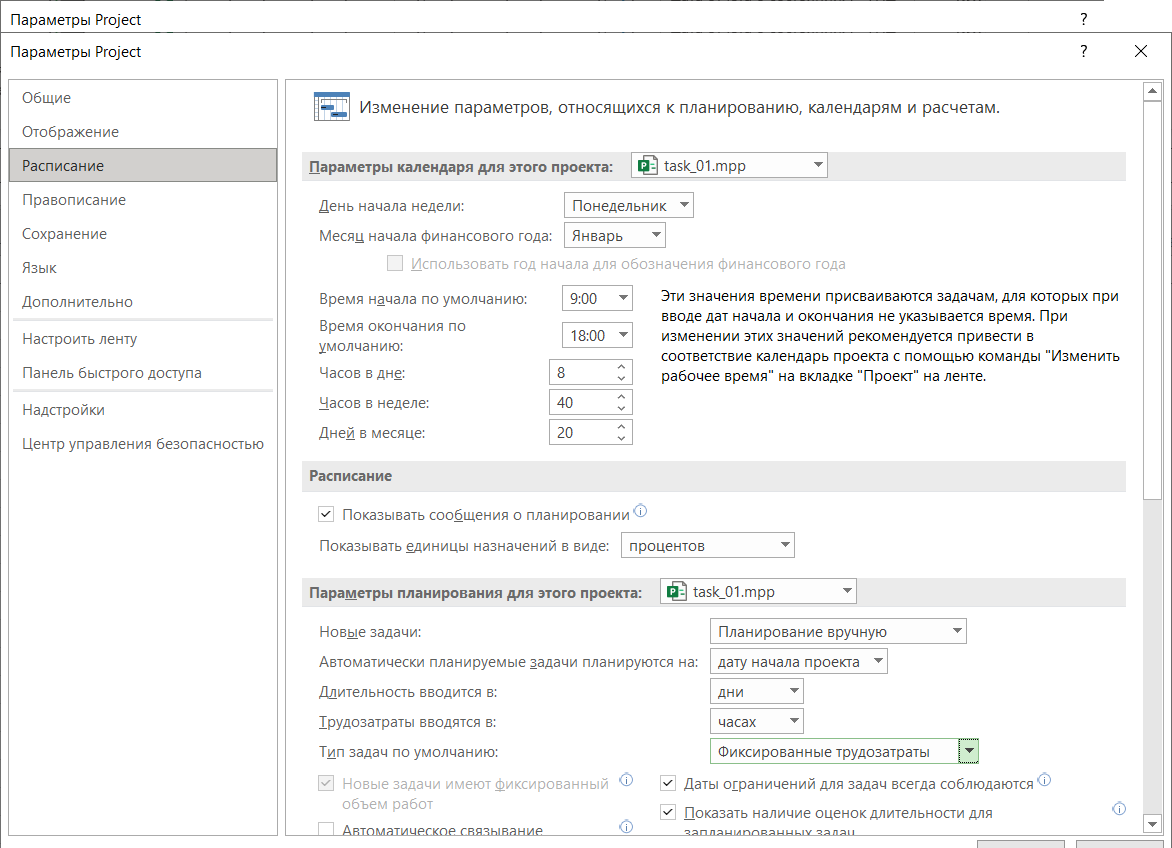
\includegraphics[width=\textwidth]{imgs/task_1_1.png}
	\end{center}
\end{figure}

Добавим праздничные дни:

\begin{figure}[H]
	\begin{center}
		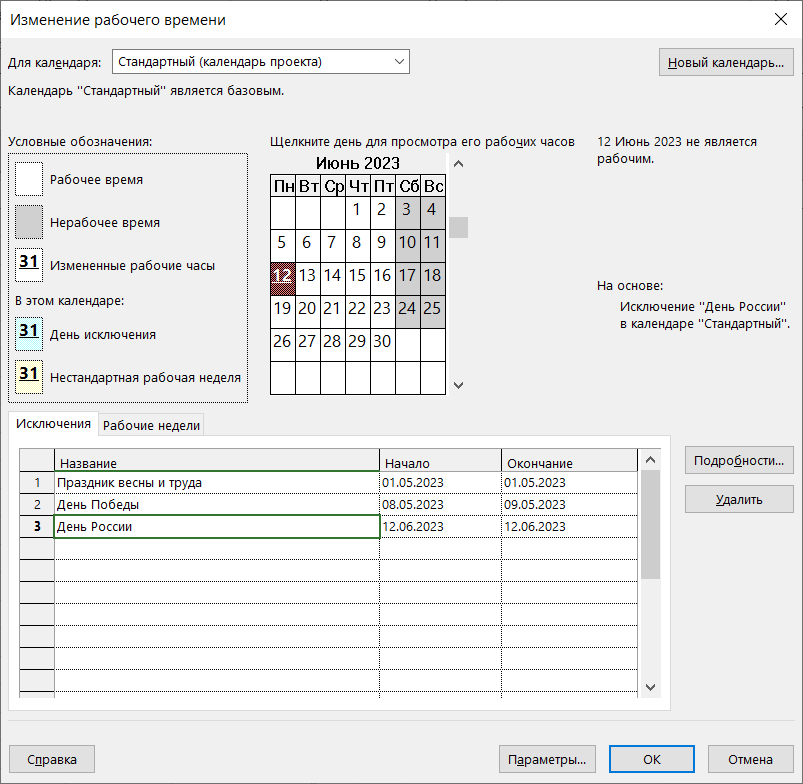
\includegraphics[width=0.7\textwidth]{imgs/task_1_2.png}
	\end{center}
\end{figure}

\section*{Задание 2: Создание списка задач}

Создадим список задач в соответствии с заданием:

\begin{figure}[H]
	\begin{center}
		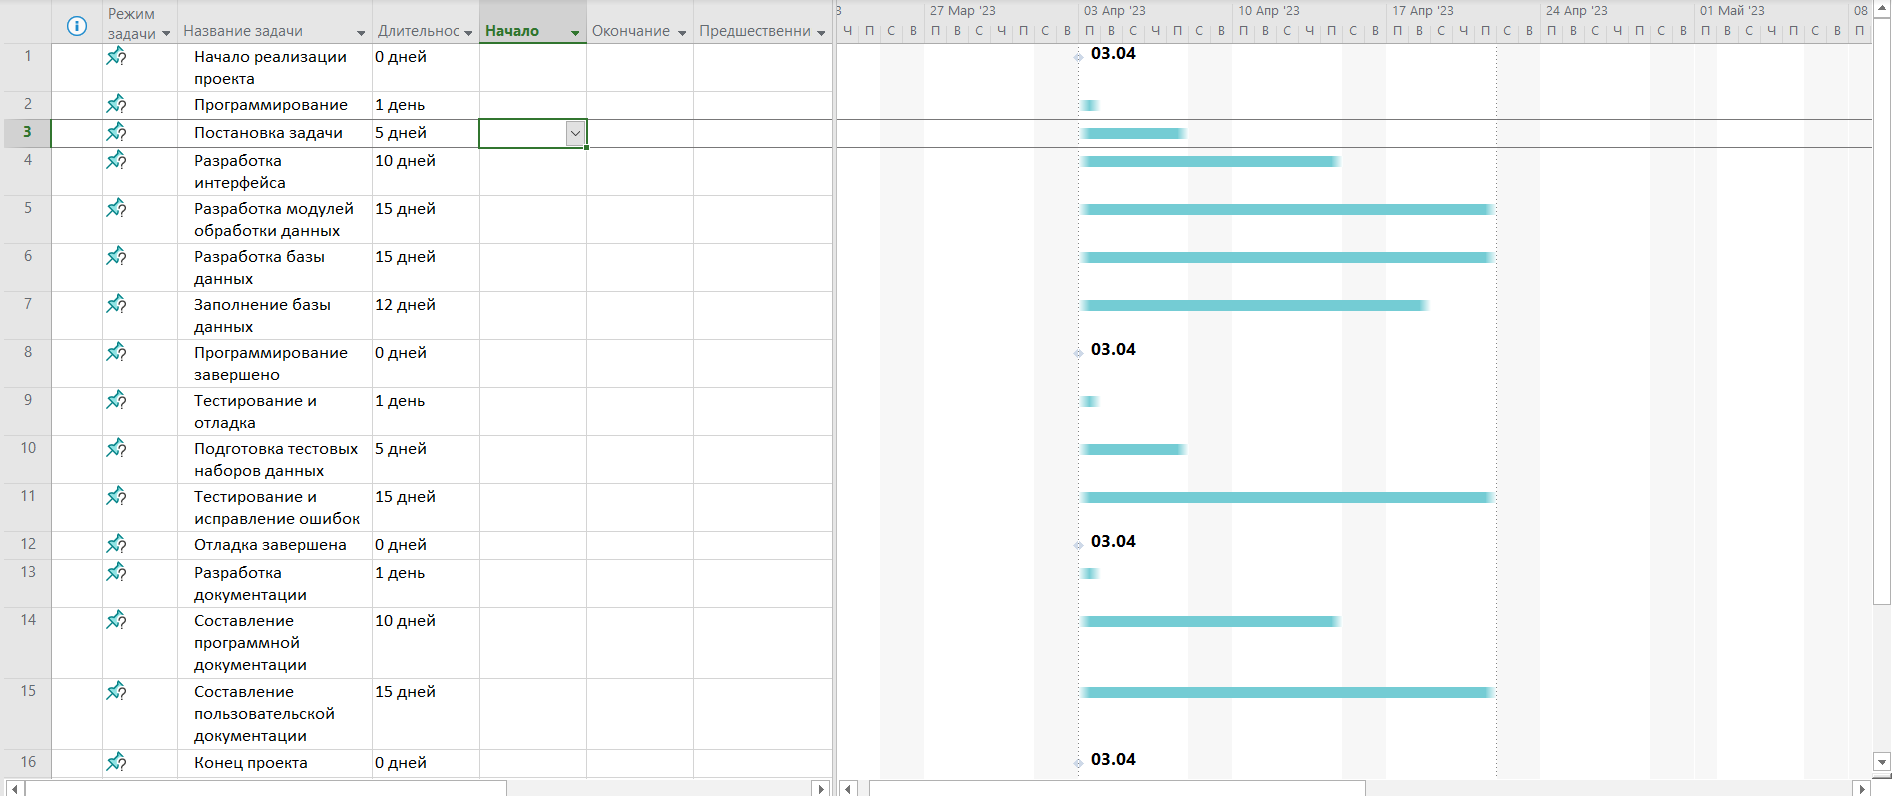
\includegraphics[width=\textwidth]{imgs/task_2_0.png}
	\end{center}
\end{figure}

\section*{Задание 3: Структурирование списка задач}

Проведем группировку задач в соответствии с заданием и настроим автоматическое планирование:

\begin{figure}[H]
	\begin{center}
		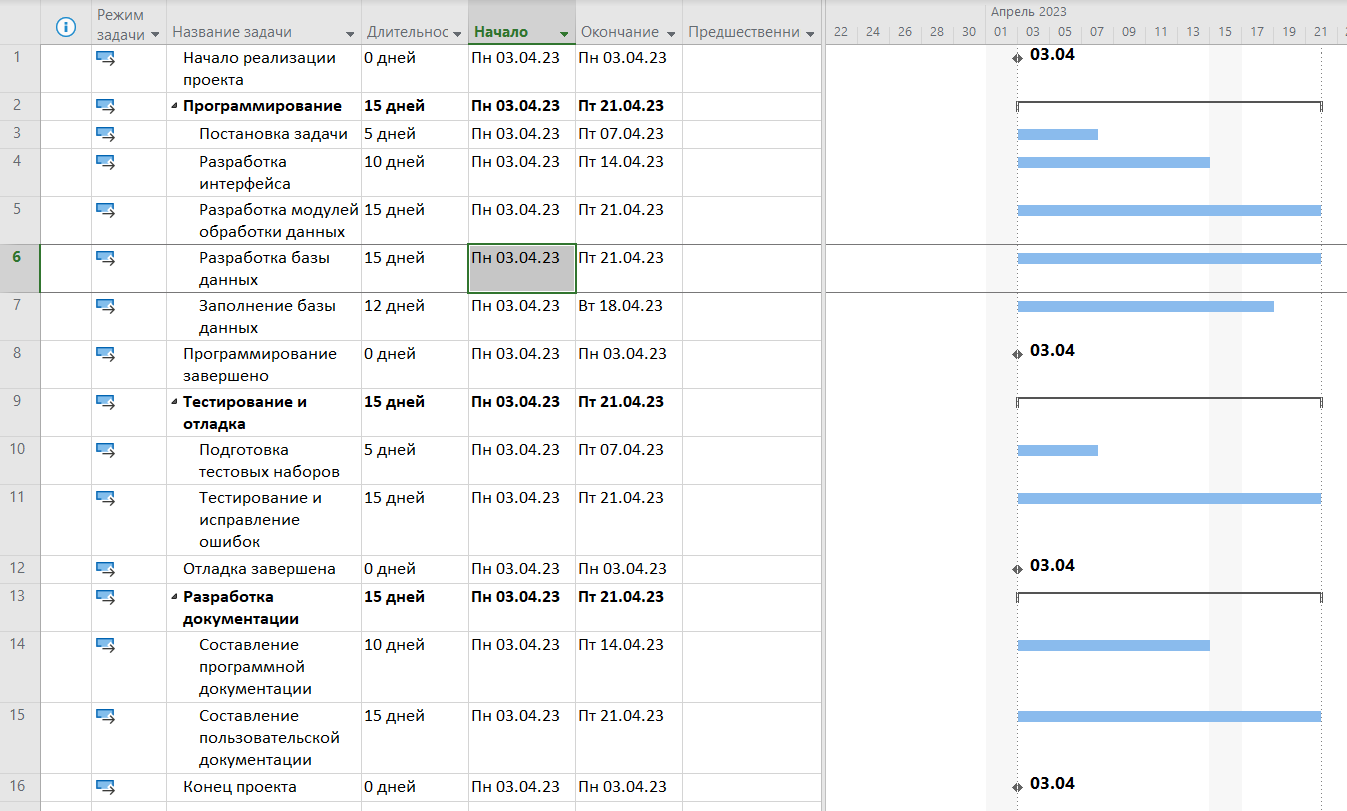
\includegraphics[width=\textwidth]{imgs/task_3_0.png}
	\end{center}
\end{figure}

\section*{Задание 4: Установка связей между задачами}

Установим связи в соответствии с заданием:

\begin{figure}[H]
	\begin{center}
		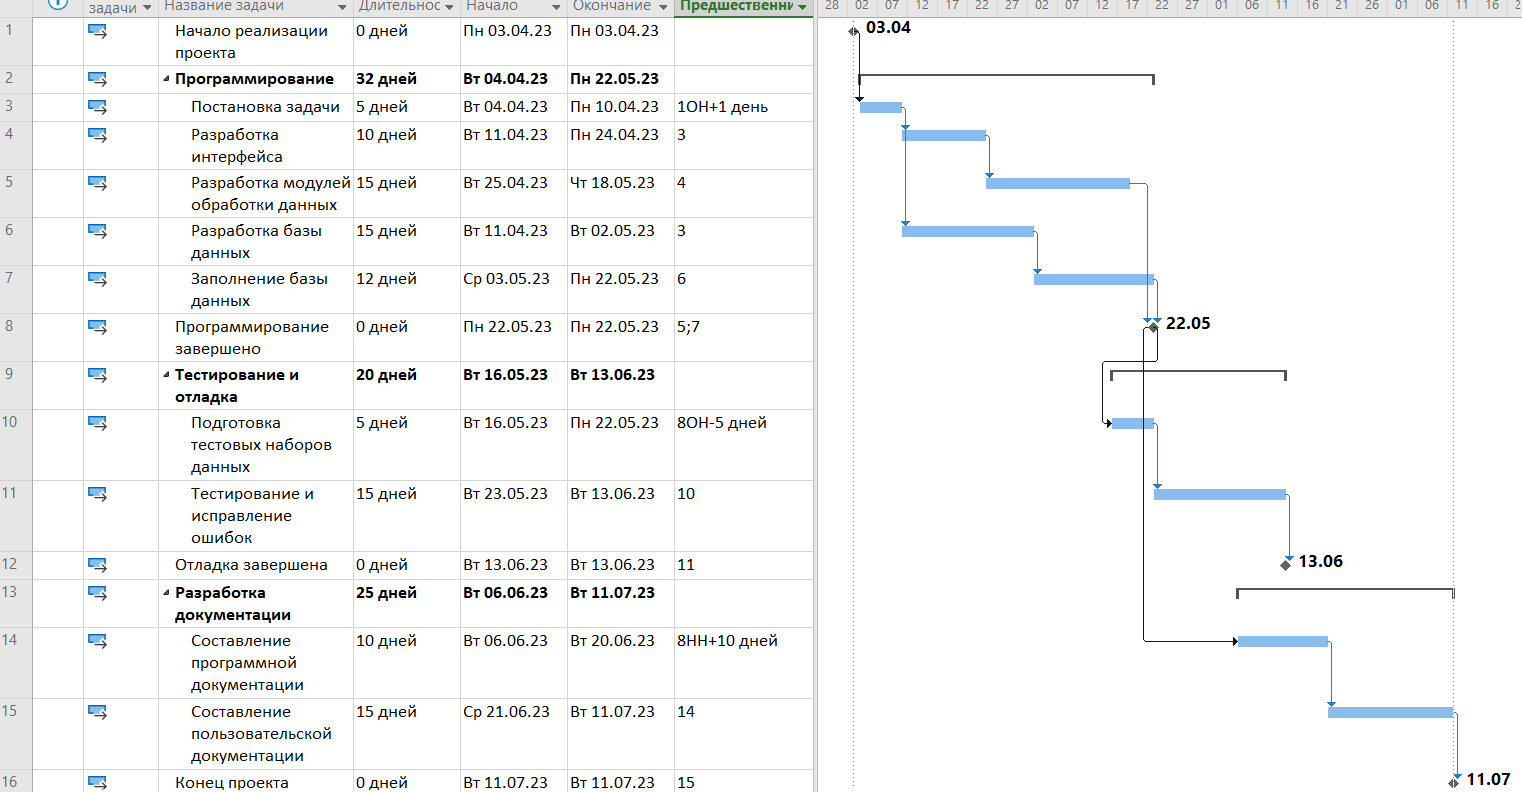
\includegraphics[width=\textwidth]{imgs/task_4_0.png}
	\end{center}
\end{figure}

\section*{Задание 5: Создание списка ресурсов}

Создадим список ресурсов в соответствии с заданием:

\begin{figure}[H]
	\begin{center}
		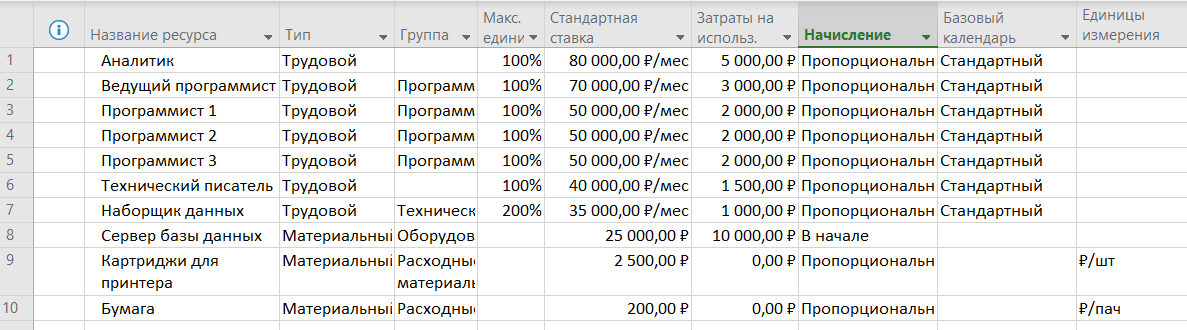
\includegraphics[width=\textwidth]{imgs/task_5_0.png}
	\end{center}
\end{figure}

Учтем, что расход бумаги -- 1 пачка в месяц, а картриджей -- 2 штуки в месяц:

\begin{figure}[H]
	\begin{center}
		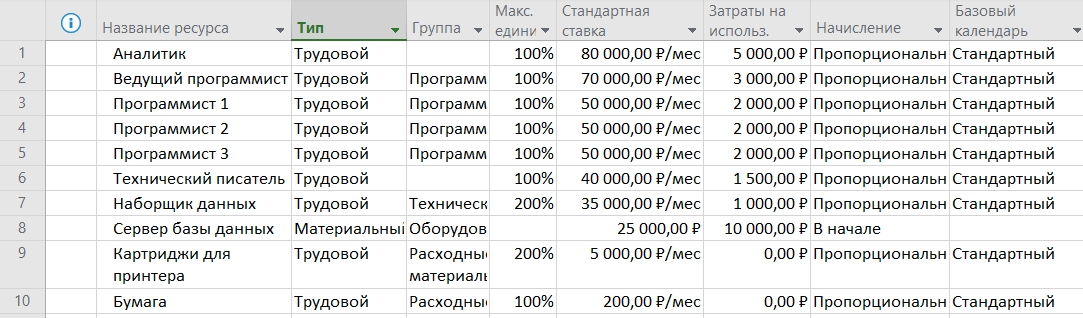
\includegraphics[width=\textwidth]{imgs/task_5_1.png}
	\end{center}
\end{figure}

\section*{Задание 6: Назначение ресурсов задачам}

Назначим ресурсы задачам в соответствии с заданием:

\begin{figure}[H]
	\begin{center}
		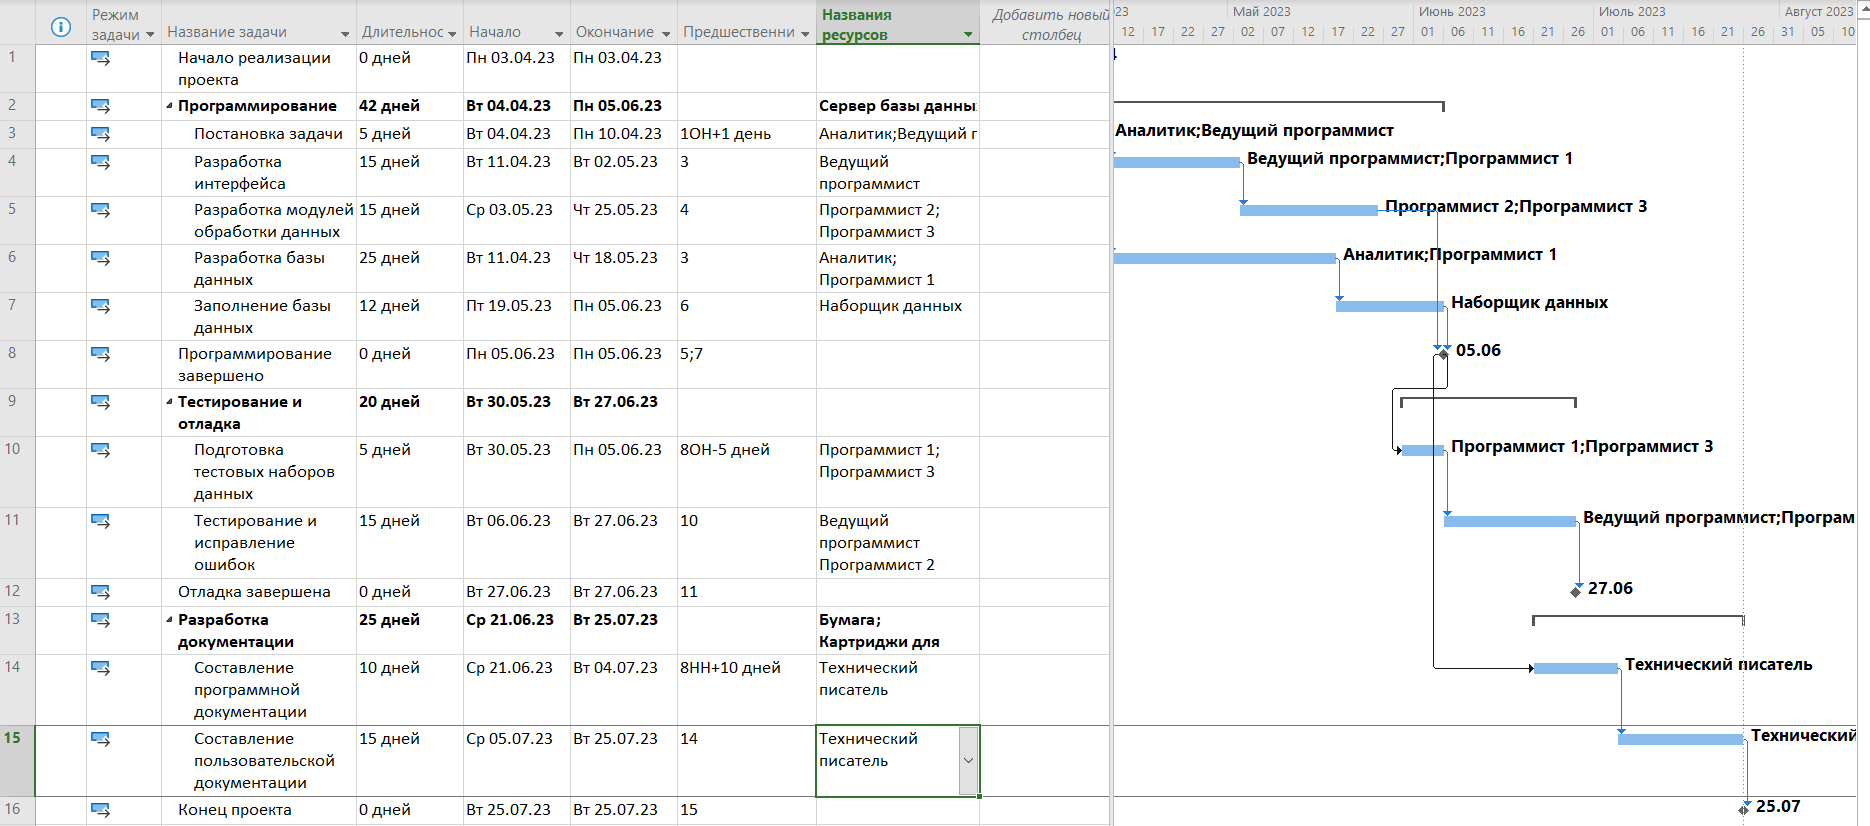
\includegraphics[width=\textwidth]{imgs/task_6_0.png}
	\end{center}
\end{figure}

Установим фиксированные затраты:

\begin{figure}[H]
	\begin{center}
		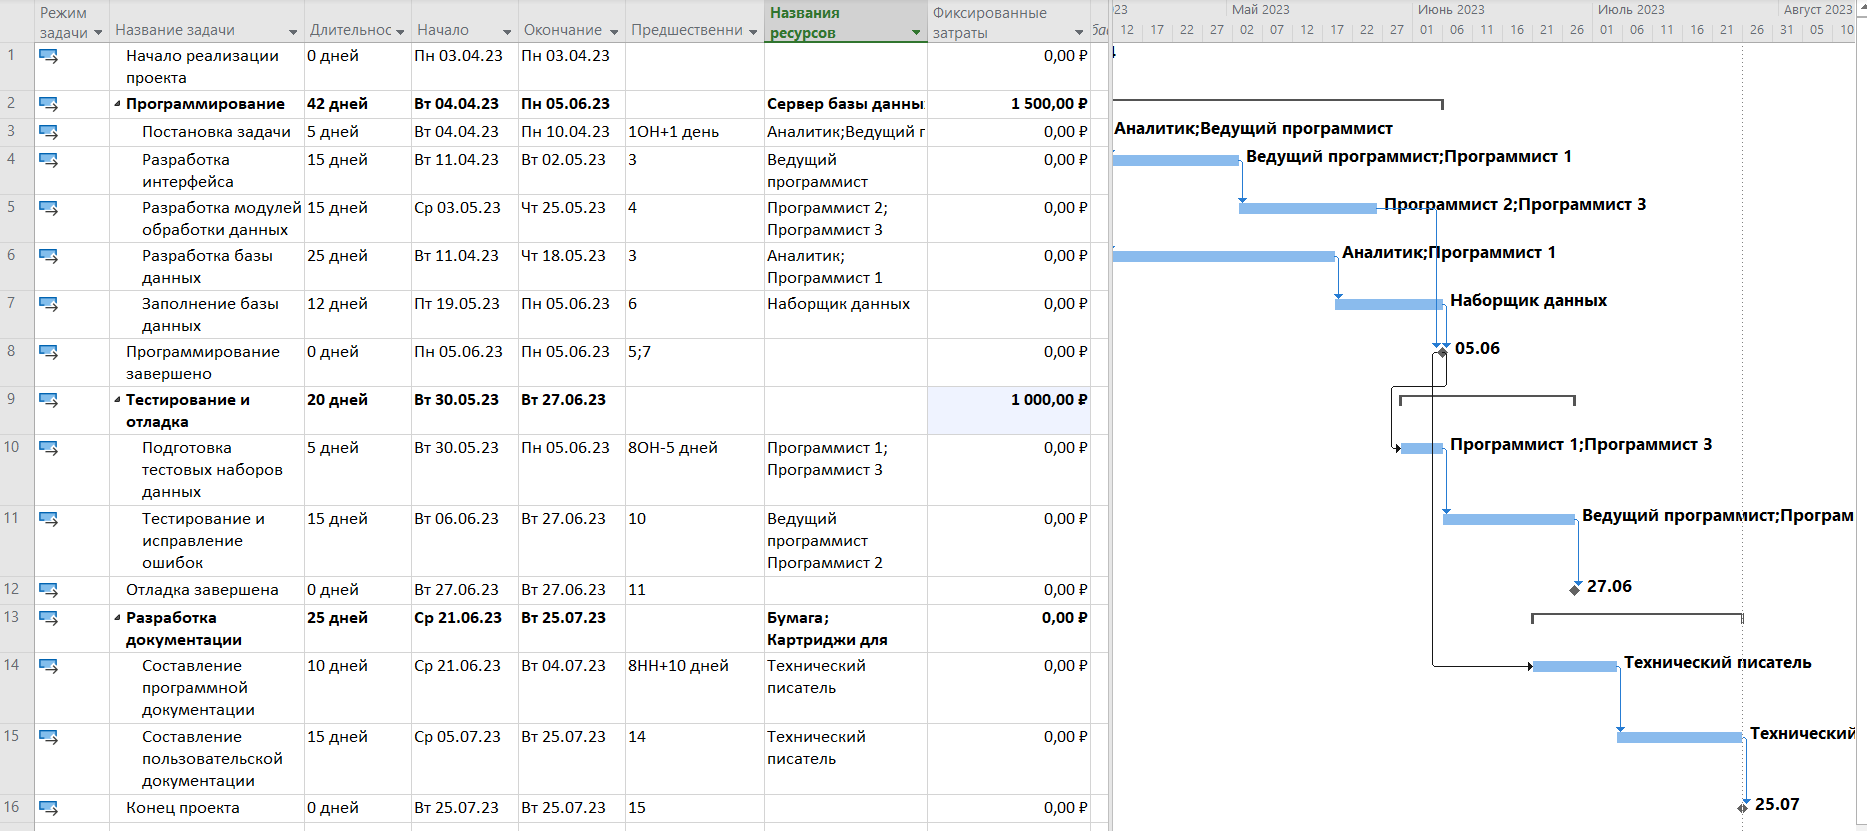
\includegraphics[width=\textwidth]{imgs/task_6_1.png}
	\end{center}
\end{figure}

\section*{Задание 7: Выравнивание загрузки ресурсов}

Можно увидеть, что перегружены 2 программиста:

\begin{figure}[H]
	\begin{center}
		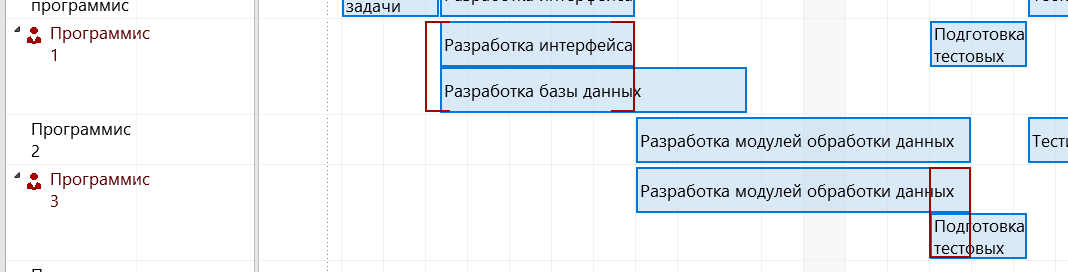
\includegraphics[width=\textwidth]{imgs/task_7_0.png}
	\end{center}
\end{figure}

Применим выравнивание. Параметры выравнивания:

\begin{figure}[H]
	\begin{center}
		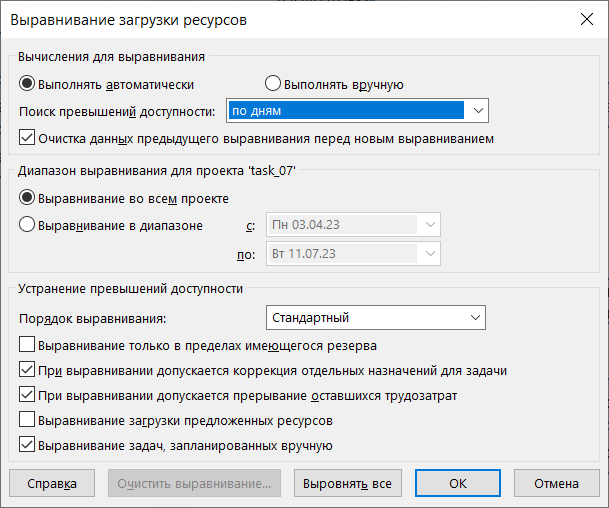
\includegraphics[width=0.7\textwidth]{imgs/task_7_1.png}
	\end{center}
\end{figure}

В результате была ликвидирована перегрузка ресурсов:

\begin{figure}[H]
	\begin{center}
		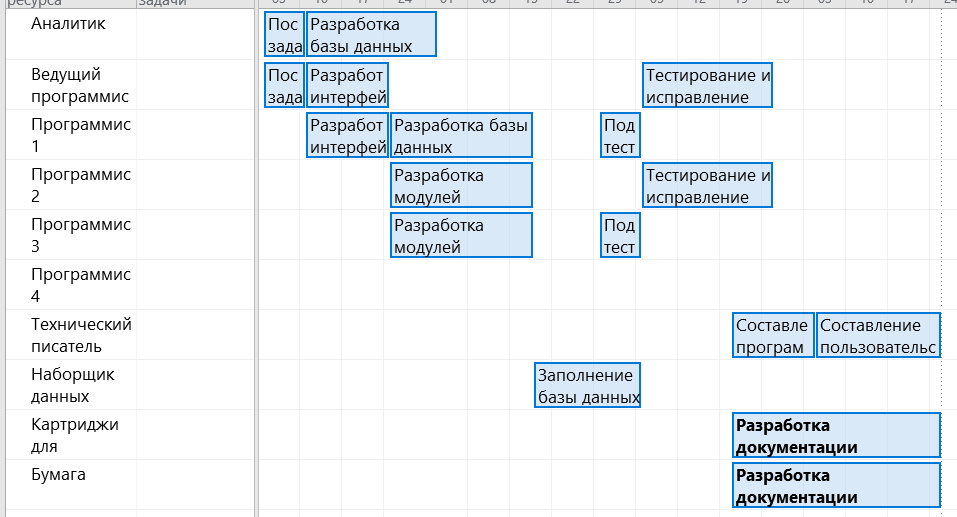
\includegraphics[width=\textwidth]{imgs/task_7_2.png}
	\end{center}
\end{figure}

\section*{Задание 8: Включение периодической задачи в план проекта}

Добавим повторяющуюся задачу <<Профилактика оборудования>>:

\begin{figure}[H]
	\begin{center}
		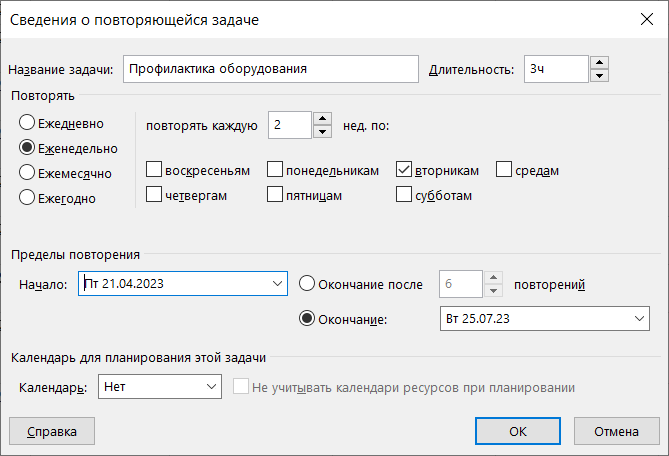
\includegraphics[width=0.7\textwidth]{imgs/task_8_0.png}
	\end{center}
\end{figure}

Учтем договор с аутсорсинговой организацией:

\begin{figure}[H]
	\begin{center}
		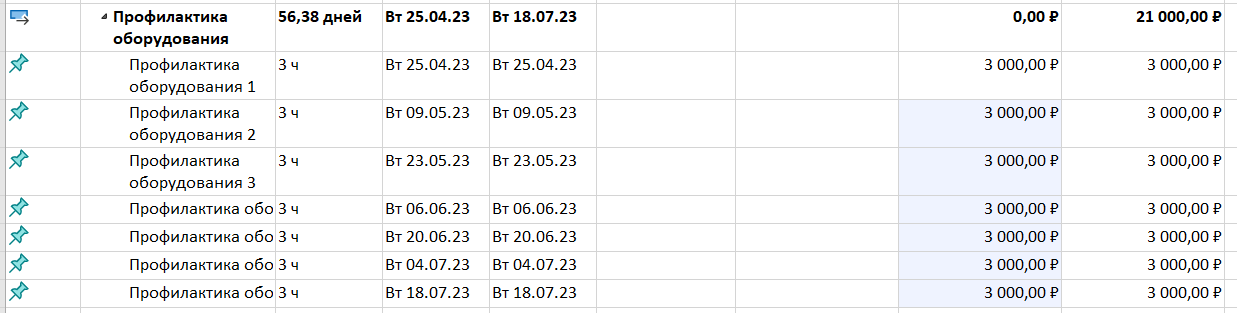
\includegraphics[width=\textwidth]{imgs/task_8_1.png}
	\end{center}
\end{figure}

Предусмотрим, что во время профилактики оборудования другие задачи не выполняются. Для этого добавим их в календарь и учтем их продолжительность:

\begin{figure}[H]
	\begin{center}
		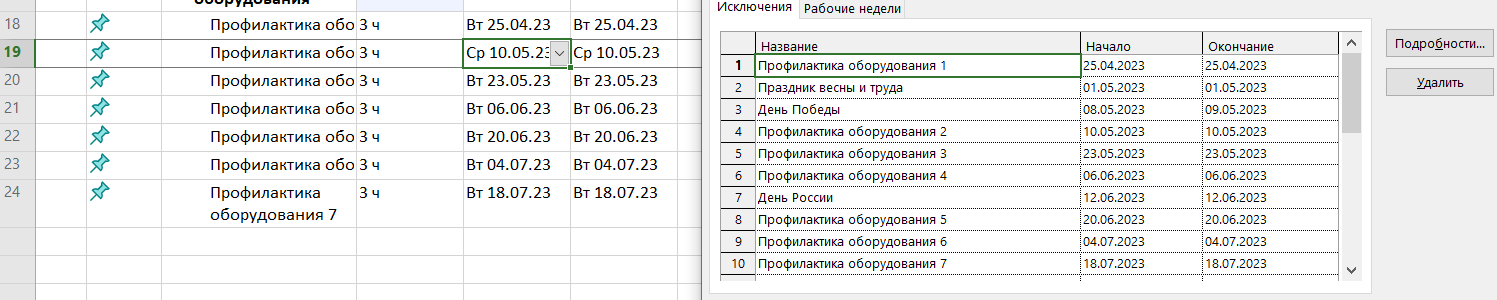
\includegraphics[width=\textwidth]{imgs/task_8_2.png}
	\end{center}
\end{figure}

\begin{figure}[H]
	\begin{center}
		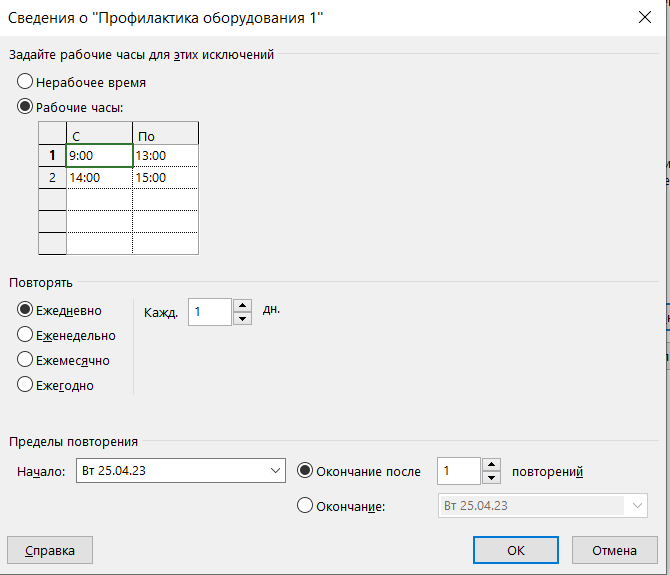
\includegraphics[width=0.7\textwidth]{imgs/task_8_3.png}
	\end{center}
\end{figure}

<<Профилактика оборудования 2>> была перенесена на 10 мая, т. к. совпадала с выходным днем (9 мая).

\section*{Задание 9: Уточнение плана проекта}

Критический путь:

\begin{figure}[H]
	\begin{center}
		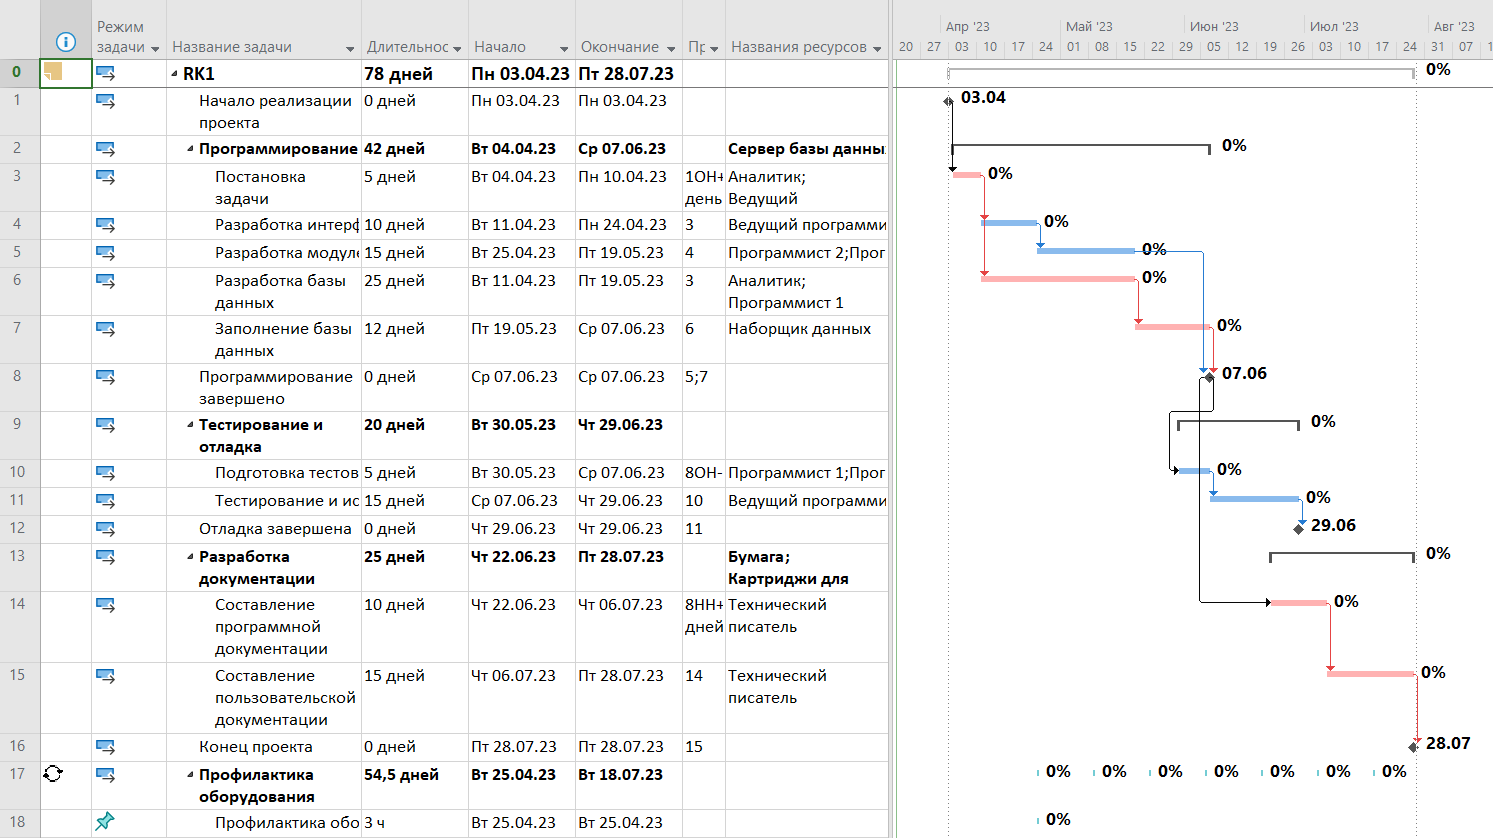
\includegraphics[width=\textwidth]{imgs/task_9_0.png}
	\end{center}
\end{figure}

До оптимизации:

\begin{figure}[H]
	\begin{center}
		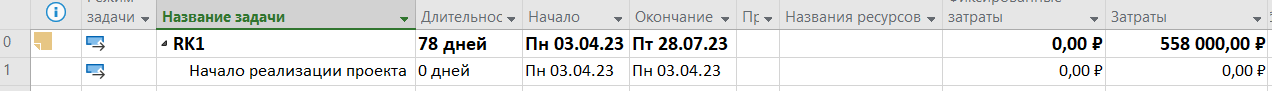
\includegraphics[width=\textwidth]{imgs/task_9_1.png}
	\end{center}
\end{figure}

В качестве оптимизации было решено добавить всех программистов в разработку базы данных:

\begin{figure}[H]
	\begin{center}
		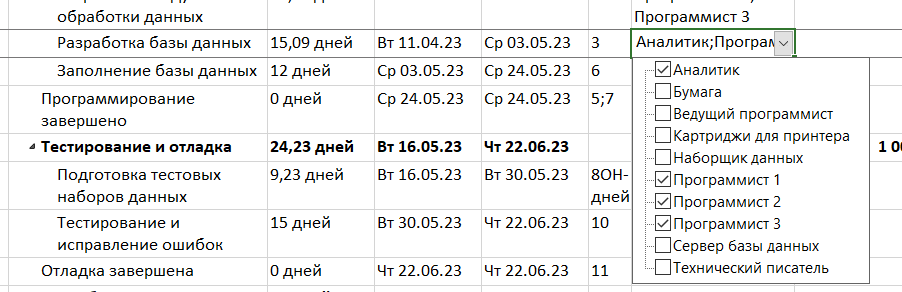
\includegraphics[width=\textwidth]{imgs/task_9_2.png}
	\end{center}
\end{figure}

После удаления проверки оборудования, выходящее за границы времени разработки проекта, получился следующий результат:

\begin{figure}[H]
	\begin{center}
		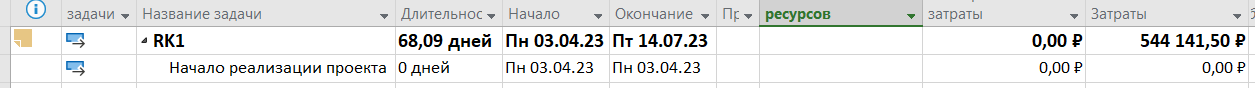
\includegraphics[width=\textwidth]{imgs/task_9_3.png}
	\end{center}
\end{figure}

В итоге получилось сократить время окончания проекта на 9.91 дней и затраты на 13858.5 рублей.

Зададим базовый план проекта:

\begin{figure}[H]
	\begin{center}
		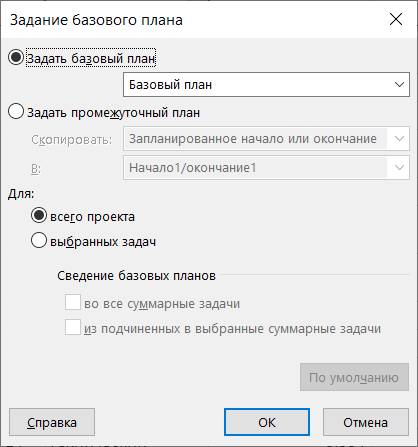
\includegraphics[width=0.5\textwidth]{imgs/task_9_4.png}
	\end{center}
\end{figure}

Проект после оптимизации:

\begin{figure}[H]
	\begin{center}
		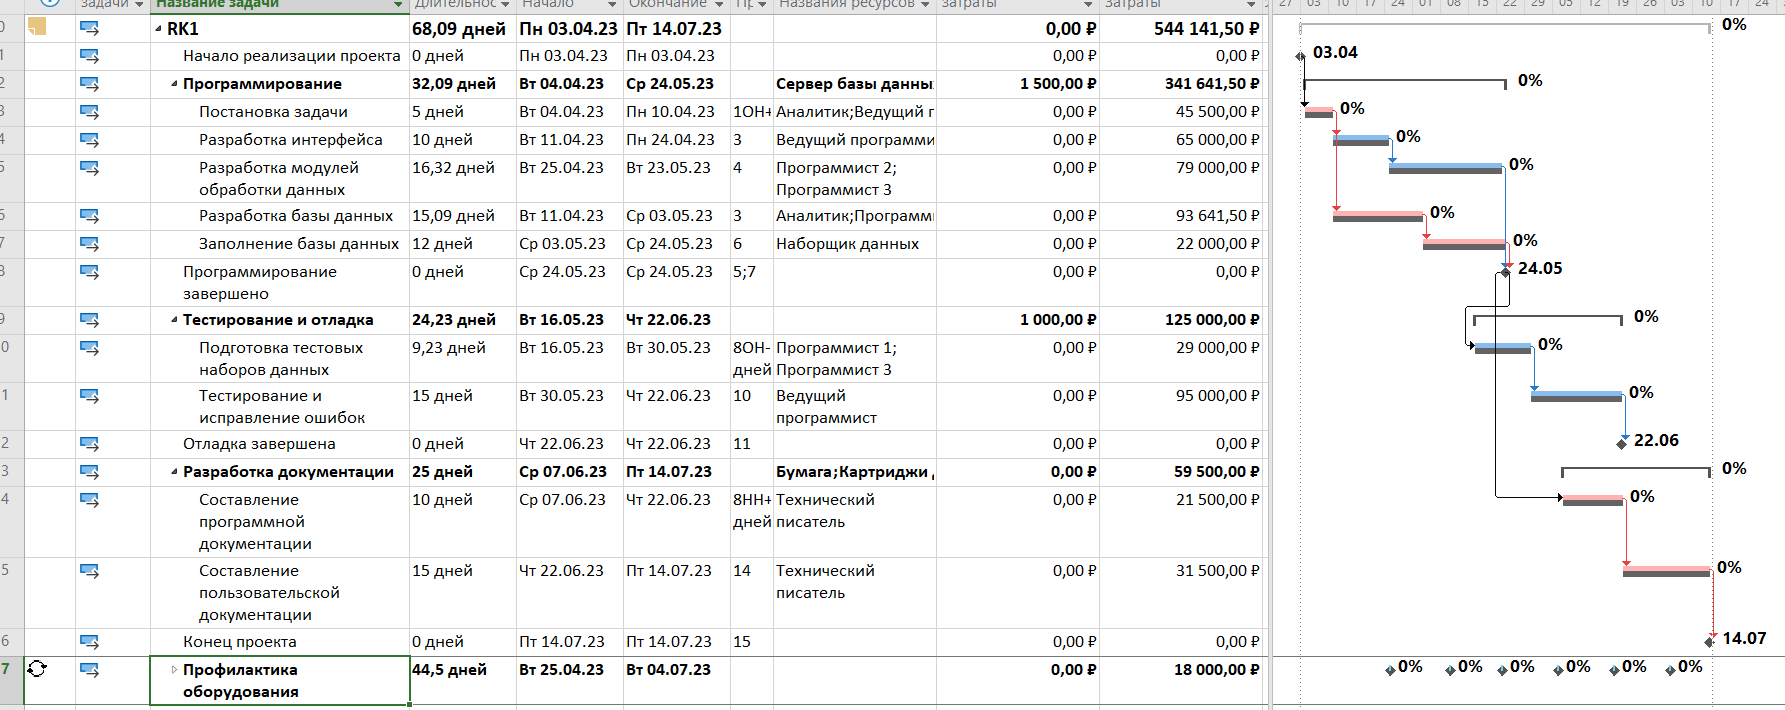
\includegraphics[width=\textwidth]{imgs/task_9_5.png}
	\end{center}
\end{figure}

\section*{Задание 10: Контроль за реализацией проекта}

Дата отчета: 1 июля.

Пусть 2 задачи задержатся на неделю:
\begin{figure}[H]
	\begin{center}
		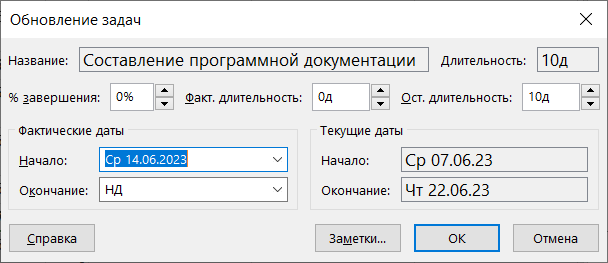
\includegraphics[width=0.7\textwidth]{imgs/task_10_0.png}
	\end{center}
\end{figure}

\begin{figure}[H]
	\begin{center}
		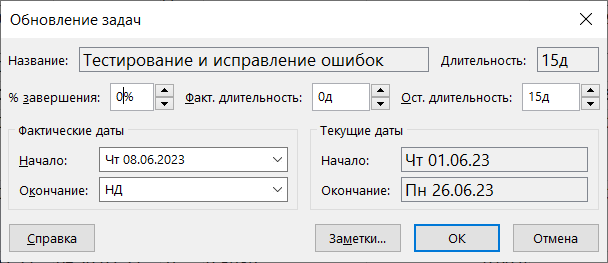
\includegraphics[width=0.7\textwidth]{imgs/task_10_1.png}
	\end{center}
\end{figure}

Бумага подорожает в полтора раза:

\begin{figure}[H]
	\begin{center}
		
\includegraphics[width=\textwidth]{imgs/task_10_2.png}
	\end{center}
\end{figure}

Постановка задачи растянется на 7 дней:

\begin{figure}[H]
	\begin{center}
		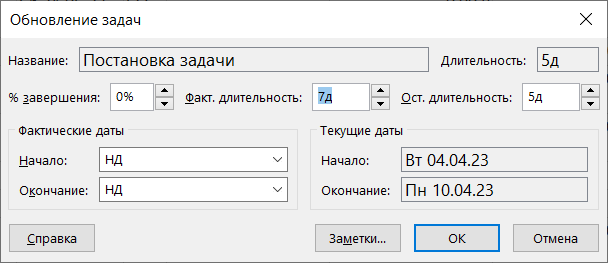
\includegraphics[width=0.7\textwidth]{imgs/task_10_3.png}
	\end{center}
\end{figure}

И заполнение базы данных растянется на 2 недели:

\begin{figure}[H]
	\begin{center}
		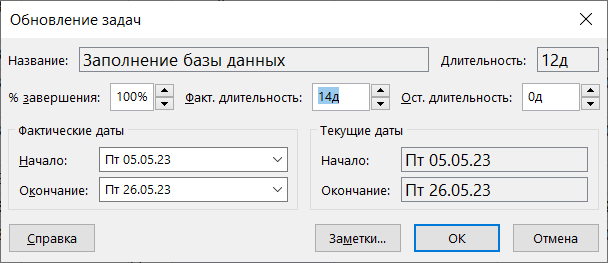
\includegraphics[width=0.7\textwidth]{imgs/task_10_4.png}
	\end{center}
\end{figure}

Фактическая длительность задачи <<Программирование>> увеличилась на 4 дня:

\begin{figure}[H]
	\begin{center}
		
\includegraphics[width=0.7\textwidth]{imgs/task_10_5.png}
	\end{center}
\end{figure}

Видно, что проект отклонился от базового плана:

\begin{figure}[H]
	\begin{center}
		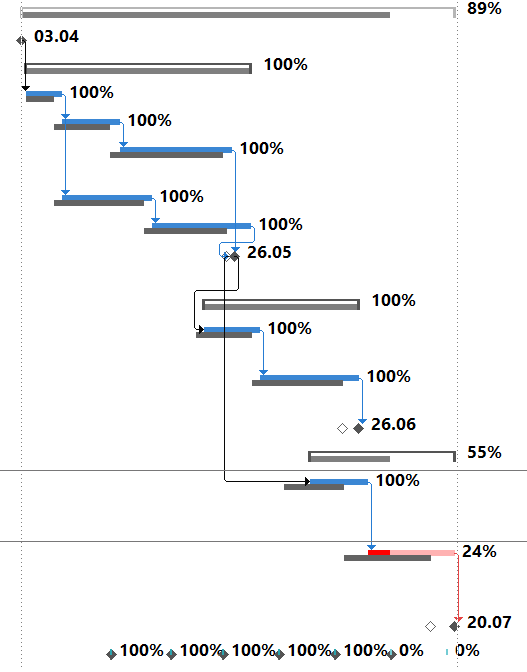
\includegraphics[width=\textwidth]{imgs/task_10_6.png}
	\end{center}
\end{figure}

Настройки линии прогресса:

\begin{figure}[H]
	\begin{center}
		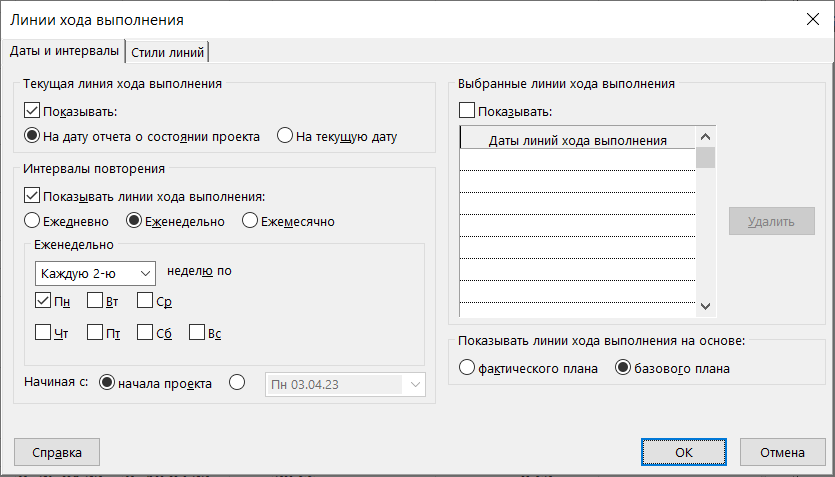
\includegraphics[width=\textwidth]{imgs/task_10_7.png}
	\end{center}
\end{figure}

Линия прогресса:

\begin{figure}[H]
	\begin{center}
		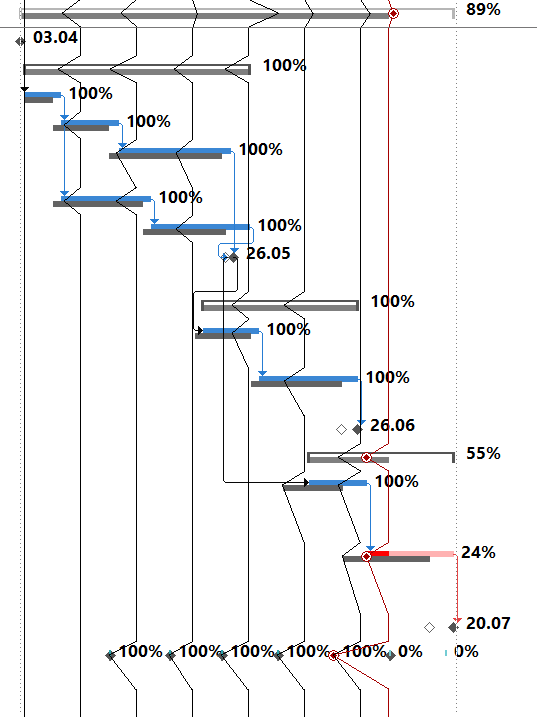
\includegraphics[width=\textwidth]{imgs/task_10_8.png}
	\end{center}
\end{figure}

Отклонение от базового плана всего проекта на момент даты отчета составляет 3.41 дней:

\begin{figure}[H]
	\begin{center}
		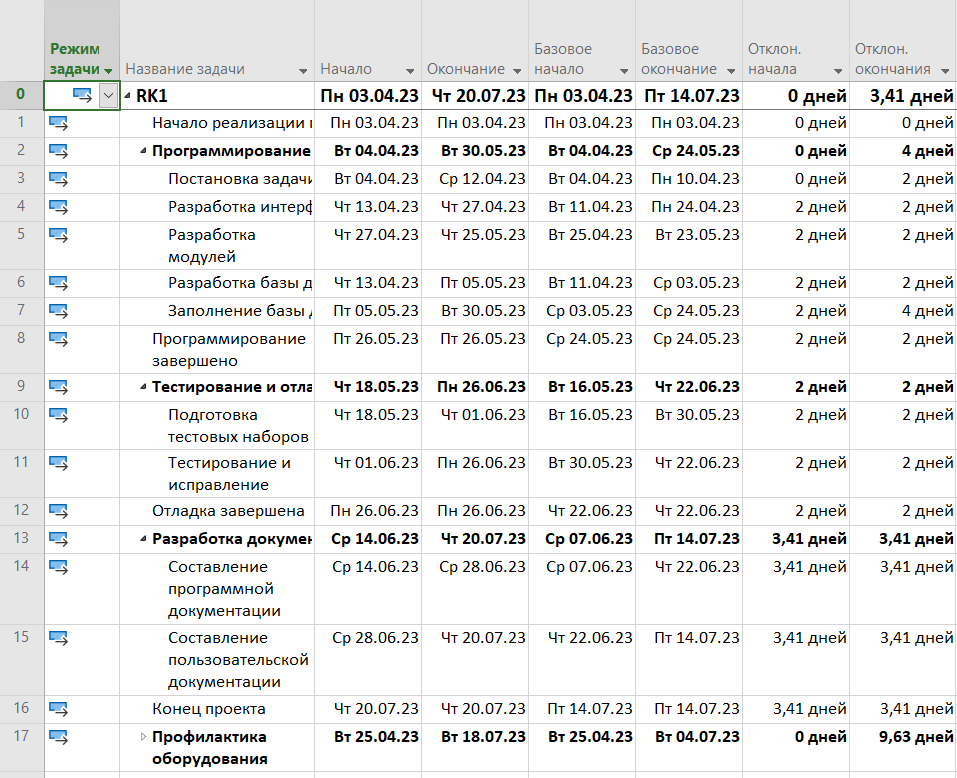
\includegraphics[width=\textwidth]{imgs/task_10_9.png}
	\end{center}
\end{figure}

Проанализируем стоимостные параметры по методике освоенного объема:

\begin{figure}[H]
	\begin{center}
		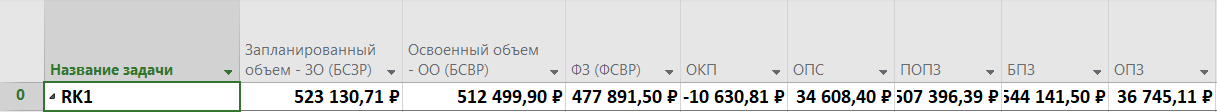
\includegraphics[width=\textwidth]{imgs/task_10_10.png}
	\end{center}
\end{figure}

\textbf{Итоговые характеристики}:

\begin{itemize}
	\item Затраты: 575766.50
	\item Длительность: 71.5 дней
	\item Окончание: 20.07.23
	\item ОКП отрицательный -- проект запаздывает;
	\item ОПС положительный -- проекту можно выделить дополнительные ресурсы, чтобы ликвидировать отставание;
	\item ОПЗ положительный -- проект укладывается в смету.
\end{itemize}

Вывод: проект укладывается в бюджет (620  тыс. руб.) и, если выделить дополнительные ресурсы, можно уложиться в срок.